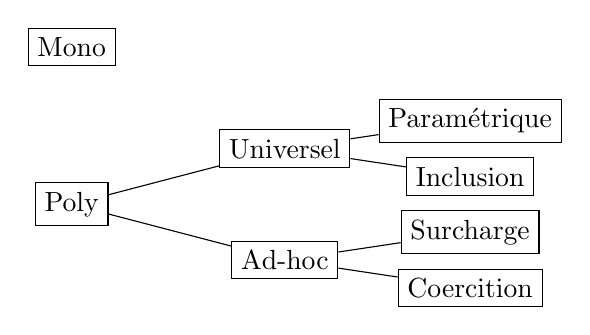
\begin{tikzpicture}
  [ ptype/.style={draw=black,shape=rectangle}
  , child/.style={ptype, xshift=2cm}
  , gen0/.style={       node distance=2cm}
  , gen1/.style={child, node distance=1cm}
  , gen2/.style={child, node distance=5mm}
  ]

  \node[ptype]                     (mono) {Mono};
  \node[ptype,below of=mono, gen0] (poly) {Poly};
  \node[above right of=poly, gen1] (univ)  {Universel};
  \node[above right of=univ, gen2] (param) {Paramétrique};
  \node[below right of=univ, gen2] (inclu) {Inclusion};
  \node[below right of=poly, gen1] (adho)  {Ad-hoc};
  \node[above right of=adho, gen2] (over)  {Surcharge};
  \node[below right of=adho, gen2] (coer)  {Coercition};

  \draw (poly) -- (univ);
  \draw (poly) -- (adho);

  \draw (univ) -- (param);
  \draw (univ) -- (inclu);

  \draw (adho) -- (over);
  \draw (adho) -- (coer);

      %node {Mono}
      %node {Poly}
          %node {Universal}
              %node {Param}
              %node {Inclusion}
          %node {Ad-Hoc}
              %node {Surcharge}
              %node {Coercition}

\end{tikzpicture}
